\lecture_date{25/10/2026}
\chapter{Lecture 04}

In the previous lecture, we started reviewing multivariable calculus. We will return to it when we study multivariable optimisation. For now, we introduce some terminology and study optimisation of smooth functions of one variable.

\section{Terminology related to optimisation}

Our basic minimisation problem is
\begin{equation}
	\min_{\mathbf{x}\in S} f(\mathbf{x}),
	\qquad f:\mathrm{Dom}\,f\to\mathbb{R},
	\qquad \varnothing\neq S\subseteq\mathrm{Dom}\,f\subseteq\mathbb{R}^n.
	\label{eq:lec04-optimisation-problem}
\end{equation}
Here, we choose an input from $S$ so that the value of $f$ is as small as possible. Notice that $S$ need not be the entire domain of $f$.

\begin{definition}[Objective function and feasible set]
	The function $f$ that we want to optimise is called the \emph{objective function}. The set $S$ of allowed inputs is called the \emph{feasible set}. An input $\mathbf{x}\in S$ is called a \emph{feasible point}.
\end{definition}

\begin{example}
	Suppose $x_1$ and $x_2$ represent quantities of nuts and bolts, and their cost is given by the function
	\[
		f(x_1,x_2)=5x_1^2+x_2^2.
	\]
	The formula makes sense for every $(x_1,x_2)\in\mathbb{R}^2$. However, negative quantities do not make sense in this context. Thus, we may use the feasible set
	\[
		S=\{(x_1,x_2)\in\mathbb{R}^2:x_1\geq0,\ x_2\geq0\}.
	\]
	The feasible set records the restrictions on the inputs; the formula for $f$ alone does not.
\end{example}

\begin{definition}[Optimiser and optimum value]
	A point $\mathbf{x}^*\in S$ satisfying
	\begin{equation}
		f(\mathbf{x}^*)\leq f(\mathbf{x})
		\qquad\text{for every }\mathbf{x}\in S
		\label{eq:lec04-global-minimum}
	\end{equation}
	is called a \emph{minimiser}. The corresponding value $f(\mathbf{x}^*)$ is called the \emph{minimum value}. For maximisation, the inequality is reversed, and we use the terms \emph{maximiser} and \emph{maximum value}. In general, the input $\mathbf{x}^*$ is an \emph{optimiser}, whereas the output $f(\mathbf{x}^*)$ is an \emph{optimum value}.
\end{definition}

The distinction is important: an optimiser is a point in the feasible set, while an optimum value is a real number. Also, a feasible point is not necessarily an optimiser; it must satisfy the required comparison.

\subsection{Local and global extrema}

A point may give a smaller value than all nearby feasible points without giving the smallest value over the whole feasible set.

\begin{definition}[Local and global minimiser]
	Let $f:\mathrm{Dom}\,f\to\mathbb{R}$ and $S\subseteq\mathrm{Dom}\,f$. A point $\mathbf{x}^*\in S$ is a \emph{local minimiser} of $f$ over $S$ if there exists $\delta>0$ such that
	\begin{equation}
		f(\mathbf{x}^*)\leq f(\mathbf{x})
		\qquad\text{for all }\mathbf{x}\in S
		\text{ with }\|\mathbf{x}-\mathbf{x}^*\|<\delta.
		\label{eq:lec04-local-minimum}
	\end{equation}
	It is a \emph{global minimiser} if the inequality holds for every $\mathbf{x}\in S$, as in \eqref{eq:lec04-global-minimum}. The corresponding function values are called a \emph{local minimum} and the \emph{global minimum}, respectively.
\end{definition}

\begin{definition}[Local and global maximiser]
	A point $\mathbf{x}^*\in S$ is a \emph{local maximiser} if there exists $\delta>0$ such that
	\begin{equation}
		f(\mathbf{x}^*)\geq f(\mathbf{x})
		\qquad\text{for all }\mathbf{x}\in S
		\text{ with }\|\mathbf{x}-\mathbf{x}^*\|<\delta.
		\label{eq:lec04-local-maximum}
	\end{equation}
	It is a \emph{global maximiser} if the inequality holds for every $\mathbf{x}\in S$. Minima and maxima are collectively called \emph{extrema}; minimum and maximum values are \emph{optimum values}.
\end{definition}

The following schematic shows two local minimisers and one local maximiser.
\begin{center}
	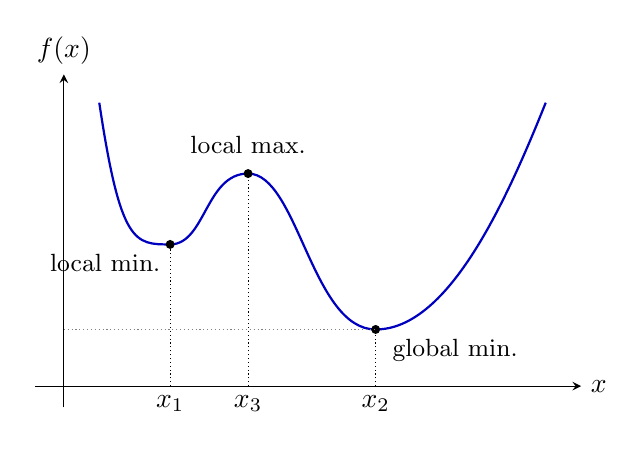
\begin{tikzpicture}[scale=0.9, >=stealth]
		\draw[->] (-0.4,0) -- (7.3,0) node[right] {$x$};
		\draw[->] (0,-0.3) -- (0,4.4) node[above] {$f(x)$};
		\draw[thick,blue!75!black]
		(0.5,4) .. controls (0.8,2) and (1,2) .. (1.5,2)
		.. controls (2,2) and (2,3) .. (2.6,3)
		.. controls (3.3,3) and (3.5,0.8) .. (4.4,0.8)
		.. controls (5.4,0.8) and (6.2,2.5) .. (6.8,4);
		\foreach \x/\y/\lab in {1.5/2/x_1,2.6/3/x_3,4.4/0.8/x_2} {
				\draw[densely dotted] (\x,0) -- (\x,\y);
				\fill (\x,\y) circle (1.8pt);
				\node[below] at (\x,0) {$\lab$};
			}
		\draw[densely dotted,gray] (0,0.8) -- (4.4,0.8);
		\node[below left] at (1.5,2) {\small local min.};
		\node[above] at (2.6,3.15) {\small local max.};
		\node[below right] at (4.5,0.8) {\small global min.};
	\end{tikzpicture}
\end{center}
Every global minimiser is a local minimiser, but the converse need not hold. Knowing the behaviour near $x_1$ does not tell us whether a lower valley exists elsewhere. This is why local information alone usually does not establish global optimality. In general, finding global minima is a hard problem.

There may be several local minimisers and several global minimisers. However, if a global minimum is attained, its \emph{value} is unique. Indeed, if $\mathbf{x}_1^*$ and $\mathbf{x}_2^*$ are global minimisers, then
\[
	f(\mathbf{x}_1^*)\leq f(\mathbf{x}_2^*)
	\quad\text{and}\quad
	f(\mathbf{x}_2^*)\leq f(\mathbf{x}_1^*).
\]
Therefore, $f(\mathbf{x}_1^*)=f(\mathbf{x}_2^*)$. The inputs can be different even though their outputs agree.

\begin{center}
	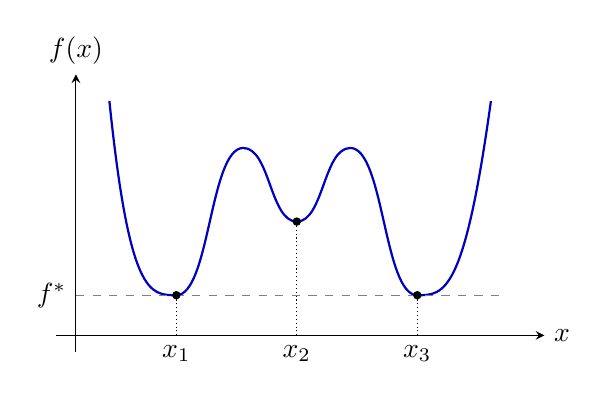
\begin{tikzpicture}[scale=0.85, >=stealth]
		\draw[->] (-0.3,0) -- (7,0) node[right] {$x$};
		\draw[->] (0,-0.25) -- (0,3.9) node[above] {$f(x)$};
		\draw[thick,blue!75!black]
		(0.5,3.5) .. controls (0.8,0.6) and (1.1,0.6) .. (1.5,0.6)
		.. controls (2,0.6) and (2,2.8) .. (2.5,2.8)
		.. controls (2.9,2.8) and (2.9,1.7) .. (3.3,1.7)
		.. controls (3.7,1.7) and (3.7,2.8) .. (4.1,2.8)
		.. controls (4.6,2.8) and (4.6,0.6) .. (5.1,0.6)
		.. controls (5.5,0.6) and (5.8,0.6) .. (6.2,3.5);
		\draw[dashed,gray] (0,0.6) -- (6.4,0.6);
		\node[left] at (0,0.6) {$f^*$};
		\foreach \x/\y/\lab in {1.5/0.6/x_1,3.3/1.7/x_2,5.1/0.6/x_3} {
				\draw[densely dotted] (\x,0) -- (\x,\y);
				\fill (\x,\y) circle (1.8pt);
				\node[below] at (\x,0) {$\lab$};
			}
	\end{tikzpicture}

	\small Three local minimisers; $x_1$ and $x_3$ share the global minimum $f^*$.
\end{center}

\subsection{The role of the feasible set}

Changing the feasible set can change both the location and the existence of an optimum, even when the objective function stays exactly the same.

\begin{example}[The same function on three feasible sets]
	Consider $f(x)=x^2$ and choose $0<a<b$.
	\begin{enumerate}
		\item If $S=\mathbb{R}$, the global minimiser is $x^*=0$ and the minimum value is $0$. There is no local or global maximum.
		\item If $S=[a,\infty)$, then $0$ is infeasible. Since $x^2$ is strictly increasing for $x>0$, the global minimiser is $a$ and the minimum value is $a^2$. There is still no global maximum.
		\item If $S=[a,b]$, the global minimiser is $a$, with value $a^2$, and the global maximiser is $b$, with value $b^2$.
	\end{enumerate}
\end{example}

\begin{center}
	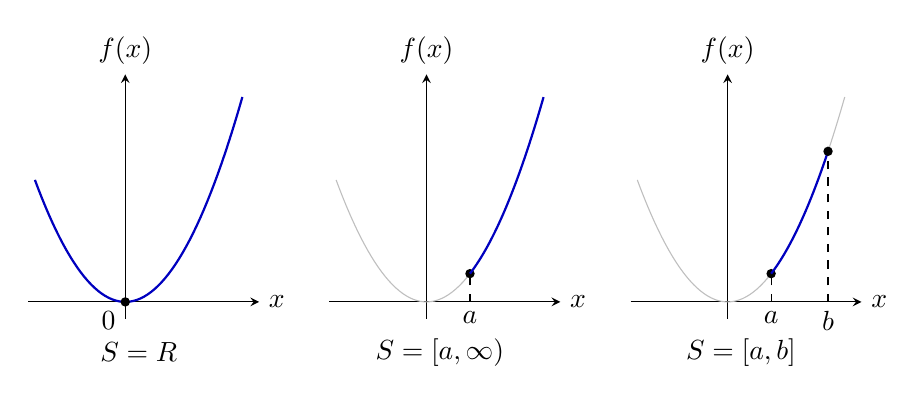
\begin{tikzpicture}[scale=0.85, >=stealth]
		\foreach \shift/\case in {0/1,4.5/2,9/3} {
				\begin{scope}[xshift=\shift cm]
					\draw[->] (-1.45,0) -- (2,0) node[right] {$x$};
					\draw[->] (0,-0.25) -- (0,3.4) node[above] {$f(x)$};
					\draw[gray!50,domain=-1.35:1.75,samples=60]
					plot (\x,{\x*\x});
					\ifnum\case=1
						\draw[thick,blue!75!black,domain=-1.35:1.75,samples=60]
						plot (\x,{\x*\x});
						\fill (0,0) circle (2pt);
						\node[below left] at (0,0) {$0$};
						\node at (0.2,-0.75) {$S=\mathbb{R}$};
					\else
						\draw[dashed] (0.65,0) -- (0.65,0.4225);
						\fill (0.65,0.4225) circle (2pt);
						\node[below] at (0.65,0) {$a$};
						\ifnum\case=2
							\draw[thick,blue!75!black,domain=0.65:1.75,samples=60]
							plot (\x,{\x*\x});
							\node at (0.2,-0.75) {$S=[a,\infty)$};
								\else
								\draw[thick,blue!75!black,domain=0.65:1.5,samples=60]
								plot (\x,{\x*\x});
								\draw[dashed] (1.5,0) -- (1.5,2.25);
								\fill (1.5,2.25) circle (2pt);
								\node[below] at (1.5,0) {$b$};
								\node at (0.2,-0.75) {$S=[a,b]$};
						\fi
					\fi
				\end{scope}
			}
	\end{tikzpicture}

	\small The blue portions correspond to feasible inputs; $0<a<b$.
\end{center}

In the terminology used in class, a \emph{natural extremum} comes from the behaviour of the function itself, without an added restriction on its domain. An \emph{induced extremum} arises because a constraint removes inputs that would otherwise prevent that point from being an extremum.

For $f(x)=x^2$, the minimum at $0$ over $\mathbb{R}$ is natural. The minimum at $a>0$ over $[a,\infty)$ is induced by the constraint. Over $[a,b]$, with $0<a<b$, both the minimum at $a$ and the maximum at $b$ are induced. They are also local extrema relative to the feasible set.

If the feasible interval includes $0$, the natural minimiser remains feasible.

\begin{definition}[Constrained and unconstrained optimisation]
	If we restrict the allowed inputs beyond the domain of the function, we have a \emph{constrained optimisation problem}. If $S=\mathrm{Dom}\,f$, so that no additional restriction is imposed, we have an \emph{unconstrained optimisation problem}.
\end{definition}

For most of the initial part of this course, we will study unconstrained problems. Constraints will be considered later. The derivative tests below concern interior points where movement in both directions is possible.

\section{Unconstrained optimisation of smooth single-variable functions}

We now consider functions $f:\mathbb{R}\to\mathbb{R}$, or more generally $f:I\to\mathbb{R}$ on an open interval $I$, with no additional constraints.

\begin{definition}[Smooth function]
	A function on an open interval is called \emph{smooth} if it has continuous derivatives of every order; that is, it can be differentiated infinitely many times.
\end{definition}

\begin{example}
	Polynomials, $e^x$, $\sin x$ and $\cos x$ are smooth on $\mathbb{R}$. A polynomial is still infinitely differentiable: after sufficiently many derivatives we obtain the zero function, which can be differentiated again. Functions such as $1/x$ and $\tan x$ are smooth on open intervals within their domains, but are not defined on all of $\mathbb{R}$.
\end{example}
\begin{nonexample}
	The function $|x|$ is not differentiable at $0$.
\end{nonexample}

\subsection{First and second derivative tests}

\begin{theorem}[First-order necessary condition]
	Let $x^*$ be an interior point of the domain of $f$, and suppose $f$ is differentiable at $x^*$. If $x^*$ is a local minimiser or a local maximiser, then
	\begin{equation}
		f'(x^*)=0.
		\label{eq:lec04-stationary}
	\end{equation}
\end{theorem}

For the smooth functions considered here, we find the \emph{critical points} by solving $f'(x)=0$. Each is only a candidate for a local optimiser and must still be checked.

\begin{theorem}[Second derivative test]
	Suppose $f$ has continuous first and second derivatives near an interior point $x^*$, and $f'(x^*)=0$.
	\begin{enumerate}
		\item If $f''(x^*)>0$, then $x^*$ is a local minimiser.
		\item If $f''(x^*)<0$, then $x^*$ is a local maximiser.
		\item If $f''(x^*)=0$, this test is inconclusive.
	\end{enumerate}
\end{theorem}

\begin{example}[The test works for $x^2$]
	Let $f(x)=x^2$. Then
	\[
		f'(x)=2x=0\iff x^*=0,
		\qquad f''(x)=2,
		\qquad f''(0)=2>0.
	\]
	Thus, $0$ is a local minimiser. In fact, $x^2\geq0=f(0)$ for all $x\in\mathbb{R}$, so $0$ is also the unique global minimiser.
\end{example}

\newpage
\begin{example}[The test is inconclusive for $x^4$]
	Let $f(x)=x^4$. Then
	\[
		f'(x)=4x^3=0\iff x^*=0,
		\qquad f''(x)=12x^2,
		\qquad f''(0)=0.
	\]
	The second derivative test gives no conclusion. Nevertheless, $x^4>0=f(0)$ for every $x\neq0$, so $0$ is the unique global minimiser. A zero second derivative does not mean there is no extremum.
\end{example}

\begin{example}[Zero first derivative does not guarantee an extremum]
	Let $f(x)=x^3$. Then
	\[
		f'(x)=3x^2=0\iff x^*=0,
		\qquad f''(x)=6x,
		\qquad f''(0)=0.
	\]
	For every $h>0$, we have $f(-h)<f(0)<f(h)$. Thus, $0$ is neither a local minimiser nor a local maximiser. The same pair of values $f'(0)=f''(0)=0$ occurs for $x^4$, but the behaviour is different.
\end{example}

\begin{center}
	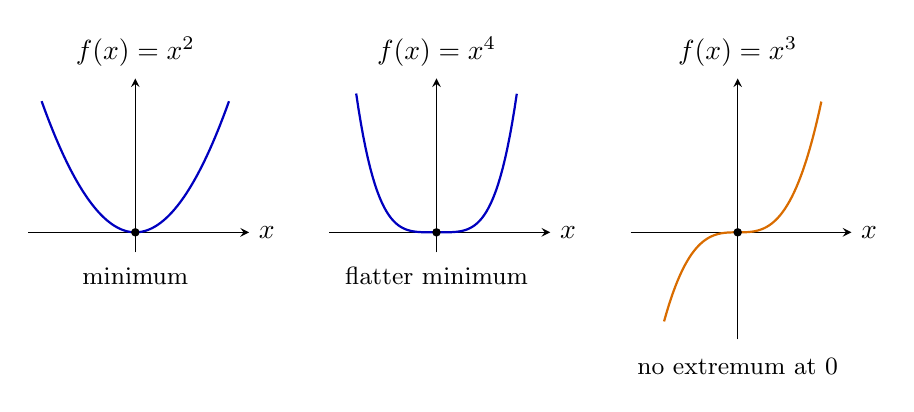
\begin{tikzpicture}[scale=0.85, >=stealth]
		\begin{scope}
			\draw[->] (-1.6,0) -- (1.7,0) node[right] {$x$};
			\draw[->] (0,-0.3) -- (0,2.3);
			\draw[thick,blue!75!black,domain=-1.4:1.4,samples=70]
			plot (\x,{\x*\x});
			\fill (0,0) circle (1.8pt);
			\node at (0,2.7) {$f(x)=x^2$};
			\node at (0,-0.65) {\small minimum};
		\end{scope}
		\begin{scope}[xshift=4.5cm]
			\draw[->] (-1.6,0) -- (1.7,0) node[right] {$x$};
			\draw[->] (0,-0.3) -- (0,2.3);
			\draw[thick,blue!75!black,domain=-1.2:1.2,samples=70]
			plot (\x,{\x*\x*\x*\x});
			\fill (0,0) circle (1.8pt);
			\node at (0,2.7) {$f(x)=x^4$};
			\node at (0,-0.65) {\small flatter minimum};
		\end{scope}
		\begin{scope}[xshift=9cm]
			\draw[->] (-1.6,0) -- (1.7,0) node[right] {$x$};
			\draw[->] (0,-1.6) -- (0,2.3);
			\draw[thick,orange!85!black,domain=-1.1:1.25,samples=70]
			plot (\x,{\x*\x*\x});
			\fill (0,0) circle (1.8pt);
			\node at (0,2.7) {$f(x)=x^3$};
			\node at (0,-2) {\small no extremum at $0$};
		\end{scope}
	\end{tikzpicture}
\end{center}

\subsection{Taylor expansion and higher derivative test}
To understand these tests, compare the value at $x^*$ with the value at a nearby point $x^*+h$. A positive $h$ moves to the right; a negative $h$ moves to the left. At a local minimum, we require
\begin{equation}
	f(x^*+h)-f(x^*)\geq0
	\qquad\text{for all sufficiently small }|h|.
	\label{eq:lec04-local-difference}
\end{equation}
At a local maximum, the difference is nonpositive.

\begin{center}
	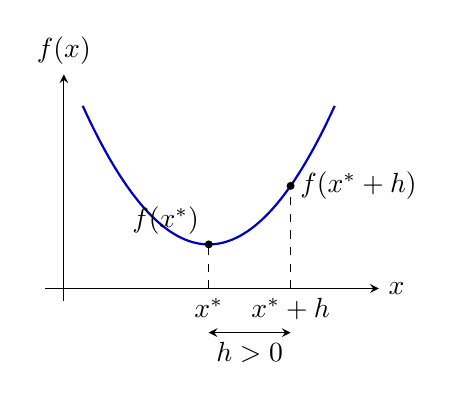
\begin{tikzpicture}[scale=0.8, >=stealth]
		\draw[->] (-2.6,0) -- (2.7,0) node[right] {$x$};
		\draw[->] (-2.3,-0.2) -- (-2.3,3.4) node[above] {$f(x)$};
		\draw[thick,blue!75!black,domain=-2:2,samples=70]
		plot (\x,{0.55*\x*\x+0.7});
		\draw[dashed] (0,0) -- (0,0.7);
		\draw[dashed] (1.3,0) -- (1.3,1.6295);
		\fill (0,0.7) circle (1.8pt);
		\fill (1.3,1.6295) circle (1.8pt);
		\node[above left] at (0,0.7) {$f(x^*)$};
		\node[right] at (1.3,1.6295) {$f(x^*+h)$};
		\node[below] at (0,0) {$x^*$};
		\node[below] at (1.3,0) {$x^*+h$};
		\draw[<->] (0,-0.7) -- (1.3,-0.7) node[midway,below] {$h>0$};
	\end{tikzpicture}
\end{center}

A function is \emph{analytic} near a point if it agrees with its Taylor series there. Smoothness alone does not guarantee this. As in the lecture, assume here that $f$ is analytic near $x^*$, so that we can write
\begin{equation}
	f(x^*+h)=f(x^*)+h f'(x^*)
	+\frac{h^2}{2!}f''(x^*)
	+\frac{h^3}{3!}f^{(3)}(x^*)+\cdots.
	\label{eq:lec04-taylor-series}
\end{equation}
Here, $f^{(k)}(x^*)$ denotes the $k$th derivative evaluated at $x^*$. Each of these evaluated derivatives is a fixed number; $h$ is the quantity that varies.

\textbf{Why must the first derivative vanish?}
Subtracting $f(x^*)$ from the Taylor expansion gives
\[
	f(x^*+h)-f(x^*)
	=h f'(x^*)+\frac{h^2}{2!}f''(x^*)+\cdots.
\]
For sufficiently small $|h|$, the first nonzero term determines the sign of this difference. If $f'(x^*)\neq0$, the leading term $h f'(x^*)$ changes sign when we move from the right of $x^*$ to the left. The difference then cannot stay nonnegative on both sides, as a local minimum requires. It cannot stay nonpositive on both sides either. Therefore, at a local optimiser we must have $f'(x^*)=0$.

\textbf{Why does the second derivative classify the point?}
When $f'(x^*)=0$, the expansion starts with
\begin{equation}
	f(x^*+h)-f(x^*)
	=\frac{h^2}{2!}f''(x^*)+\frac{h^3}{3!}f^{(3)}(x^*)+\cdots.
	\label{eq:lec04-second-order}
\end{equation}
If $f''(x^*)\neq0$, the quadratic term determines the sign for sufficiently small nonzero $h$. Since $h^2$ is positive on both sides, $f''(x^*)>0$ makes the nearby values larger, giving a local minimum. Similarly, $f''(x^*)<0$ makes them smaller, giving a local maximum.

\textbf{What if the second derivative also vanishes?}
If $f'(x^*)=f''(x^*)=0$, we look at the next terms:
\begin{equation}
	f(x^*+h)-f(x^*)
	=\frac{h^3}{3!}f^{(3)}(x^*)
	+\frac{h^4}{4!}f^{(4)}(x^*)+\cdots.
	\label{eq:lec04-third-fourth-order}
\end{equation}
If $f^{(3)}(x^*)\neq0$, the leading cubic term changes sign across $x^*$, so there is no local minimum or maximum. If $f^{(3)}(x^*)=0$ but $f^{(4)}(x^*)\neq0$, the fourth-order term comes first. Since $h^4>0$ for $h\neq0$, a positive $f^{(4)}(x^*)$ gives a local minimum and a negative value gives a local maximum. If this derivative also vanishes, we look at the next order. The rule below applies once a first nonzero derivative is found.

\begin{theorem}[First nonzero derivative test]
	Let $f$ be analytic near an interior point $x^*$, as assumed in the Taylor argument above. Suppose, for some integer $m\geq1$,
	\begin{equation}
		f^{(k)}(x^*)=0\quad(1\leq k<m),
		\qquad f^{(m)}(x^*)\neq0.
		\label{eq:lec04-first-nonzero}
	\end{equation}
	Then:
	\begin{enumerate}
		\item If $m$ is odd, $x^*$ is neither a local minimiser nor a local maximiser.
		\item If $m$ is even and $f^{(m)}(x^*)>0$, then $x^*$ is a local minimiser.
		\item If $m$ is even and $f^{(m)}(x^*)<0$, then $x^*$ is a local maximiser.
	\end{enumerate}
\end{theorem}
\begin{proof}
	In the Taylor argument above, the terms before order $m$ vanish. Thus, the first nonzero term in $f(x^*+h)-f(x^*)$ is
	\[
		\frac{h^m}{m!}f^{(m)}(x^*).
	\]
	For sufficiently small nonzero $h$, this term determines the sign. If $m$ is odd, $h^m$ changes sign between the two sides, so there can be no local minimum or maximum. If $m$ is even, $h^m$ is positive on both sides. The sign is then the sign of $f^{(m)}(x^*)$: positive gives a local minimum, and negative gives a local maximum.
\end{proof}

Once the first nonzero derivative is found, later derivatives do not affect this classification; they need not vanish. In particular, the test does not require every odd-order derivative to be zero at a local optimum.

Returning to $f(x)=x^4$, we have $f^{(3)}(x)=24x$ and $f^{(4)}(x)=24$. At $0$, the first nonzero evaluated derivative has even order $4$ and is positive, confirming a local minimum. For $f(x)=x^3$, $f^{(3)}(0)=6\neq0$ has odd order, so $0$ is neither a local minimum nor a local maximum.

\begin{remark}[The test need not finish for every smooth function]
	Being smooth does not guarantee that a first nonzero derivative will be found. For example, the smooth function
	\[
		q(x)=\begin{cases}
			e^{-1/x^2}, & x\neq0, \\
			0,          & x=0
		\end{cases}
	\]
	has $q^{(k)}(0)=0$ for every $k\geq1$. Nevertheless, $0$ is a global minimiser, since $q(0)=0$ and $q(x)>0$ for $x\neq0$. Thus, if all evaluated derivatives vanish, the higher derivative test gives no conclusion; we need another argument.
\end{remark}

\begin{example}[Cubic function]
	Find the local minima and maxima of
	\begin{equation}
		f(x)=x^3-6x^2+11x-6,
		\qquad x\in\mathbb{R}.
		\label{eq:lec04-cubic}
	\end{equation}
\end{example}

\textbf{Solution.}
First, note that
\[
	f(x)=(x-1)(x-2)(x-3).
\]
Thus, the graph crosses the $x$-axis at $1$, $2$ and $3$. To locate the possible local optimisers, we solve $f'(x)=0$.

\textbf{Step 1: Find the candidates.}
Differentiating gives
\[
	f'(x)=3x^2-12x+11.
\]
Hence,
\begin{align}
	3x^2-12x+11 & =0,\notag                            \\
	x           & =\frac{12\pm\sqrt{144-132}}{6}\notag \\
	            & =\frac{12\pm\sqrt{12}}{6}
	=2\pm\frac{\sqrt{3}}{3}
	=2\pm\frac{1}{\sqrt{3}}.
	\label{eq:lec04-cubic-stationary}
\end{align}
Following the board notation, let
\[
	x_1^*=2+\frac{1}{\sqrt{3}},
	\qquad x_2^*=2-\frac{1}{\sqrt{3}}.
\]
Notice that $x_2^*<x_1^*$.

\textbf{Step 2: Classify each candidate separately.}
We have $f''(x)=6x-12$. Therefore,
\begin{align*}
	f''(x_1^*) & =6\left(2+\frac{1}{\sqrt{3}}\right)-12
	=\frac{6}{\sqrt{3}}=2\sqrt{3}>0,                    \\
	f''(x_2^*) & =6\left(2-\frac{1}{\sqrt{3}}\right)-12
	=-\frac{6}{\sqrt{3}}=-2\sqrt{3}<0.
\end{align*}
Thus, $x_1^*$ is a local minimiser and $x_2^*$ is a local maximiser. Both classifications stop at the second derivative because it is already nonzero at each point.

\textbf{Step 3: Find the corresponding optimum values.}
Set $t=x-2$. Then
\begin{align*}
	f(2+t)
	 & =(2+t)^3-6(2+t)^2+11(2+t)-6              \\
	 & =(8+12t+6t^2+t^3)-(24+24t+6t^2)+22+11t-6 \\
	 & =t^3-t.
\end{align*}
Consequently,
\begin{align*}
	f(x_1^*) & =\left(\frac{1}{\sqrt{3}}\right)^3
	-\frac{1}{\sqrt{3}}
	=-\frac{2}{3\sqrt{3}},                         \\
	f(x_2^*) & =\left(-\frac{1}{\sqrt{3}}\right)^3
	+\frac{1}{\sqrt{3}}
	=\frac{2}{3\sqrt{3}}.
\end{align*}
These are the local minimum and local maximum \emph{values}, respectively.

\begin{center}
	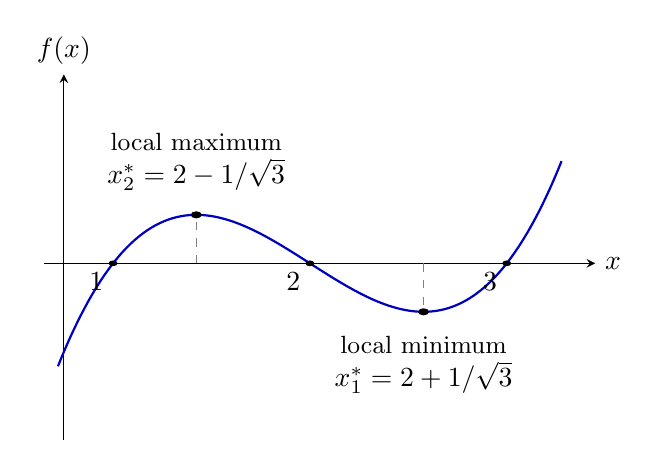
\begin{tikzpicture}[xscale=2.5,yscale=1.6, >=stealth]
		\draw[->] (0.65,0) -- (3.45,0) node[right] {$x$};
		\draw[->] (0.75,-1.4) -- (0.75,1.5) node[above] {$f(x)$};
		\draw[thick,blue!75!black,domain=0.72:3.28,samples=120]
		plot (\x,{(\x-1)*(\x-2)*(\x-3)});
		\foreach \x in {1,2,3} {
				\fill (\x,0) circle (0.65pt);
				\node[below left] at (\x,0) {$\x$};
			}
		\draw[dashed,gray] (1.42265,0) -- (1.42265,0.38490);
		\draw[dashed,gray] (2.57735,0) -- (2.57735,-0.38490);
		\fill (1.42265,0.38490) circle (0.8pt);
		\fill (2.57735,-0.38490) circle (0.8pt);
		\node[above,align=center] at (1.42265,0.5)
		{\small local maximum\\$x_2^*=2-1/\sqrt{3}$};
		\node[below,align=center] at (2.57735,-0.5)
		{\small local minimum\\$x_1^*=2+1/\sqrt{3}$};
	\end{tikzpicture}
\end{center}

\textbf{Step 4: Check whether the extrema are global.}
Since the leading term is $x^3$,
\[
	\lim_{x\to\infty}f(x)=\infty,
	\qquad \lim_{x\to-\infty}f(x)=-\infty.
\]
Thus, on $S=\mathbb{R}$ the function has neither a global minimiser nor a global maximiser. The two points found above give only local extrema. As a check, $f'(x)=3(x-x_2^*)(x-x_1^*)$ is positive before $x_2^*$, negative between $x_2^*$ and $x_1^*$, and positive after $x_1^*$. The graph therefore increases, decreases, and then increases again, consistent with the classifications above.

Different candidate points may require different numbers of derivatives. At each candidate, we stop at the first nonzero \emph{evaluated} derivative; the derivative function need not be identically zero.

Finally, interior differentiability is essential for the necessary condition $f'(x^*)=0$. For example, $|x|$ has a minimum at $0$, where the derivative does not exist. Similarly, $x^2$ on $[a,\infty)$ with $a>0$ has its minimum at $a$, although $f'(a)=2a\neq0$. At a constrained boundary, we cannot move in both directions while remaining feasible, so the argument for \eqref{eq:lec04-stationary} does not apply. We will study the appropriate conditions for constrained optimisation later.
